\documentclass[14pt]{extbook}
\usepackage{multicol, enumerate, enumitem, hyperref, color, soul, setspace, parskip, fancyhdr} %General Packages
\usepackage{amssymb, amsthm, amsmath, latexsym, units, mathtools} %Math Packages
\everymath{\displaystyle} %All math in Display Style
% Packages with additional options
\usepackage[headsep=0.5cm,headheight=12pt, left=1 in,right= 1 in,top= 1 in,bottom= 1 in]{geometry}
\usepackage[usenames,dvipsnames]{xcolor}
\usepackage{dashrule}  % Package to use the command below to create lines between items
\newcommand{\litem}[1]{\item#1\hspace*{-1cm}\rule{\textwidth}{0.4pt}}
\pagestyle{fancy}
\lhead{Progress Quiz 7}
\chead{}
\rhead{Version A}
\lfoot{4173-5738}
\cfoot{}
\rfoot{Spring 2021}
\begin{document}

\begin{enumerate}
\litem{
Construct the lowest-degree polynomial given the zeros below. Then, choose the intervals that contain the coefficients of the polynomial in the form $ax^3+bx^2+cx+d$.\[ -7, \frac{7}{2}, \text{ and } \frac{1}{2} \]\begin{enumerate}[label=\Alph*.]
\item \( a \in [-3, 6], b \in [-47, -42], c \in [117, 124], \text{ and } d \in [-51, -39] \)
\item \( a \in [-3, 6], b \in [-18, -15], c \in [-100, -89], \text{ and } d \in [48, 54] \)
\item \( a \in [-3, 6], b \in [-15, -8], c \in [-109, -101], \text{ and } d \in [-51, -39] \)
\item \( a \in [-3, 6], b \in [12, 17], c \in [-109, -101], \text{ and } d \in [48, 54] \)
\item \( a \in [-3, 6], b \in [12, 17], c \in [-109, -101], \text{ and } d \in [-51, -39] \)

\end{enumerate} }
\litem{
Which of the following equations \textit{could} be of the graph presented below?
\begin{center}
    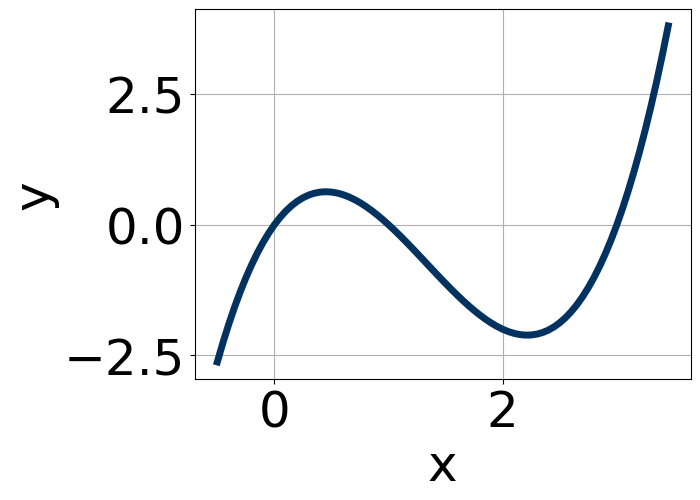
\includegraphics[width=0.5\textwidth]{../Figures/polyGraphToFunctionA.png}
\end{center}
\begin{enumerate}[label=\Alph*.]
\item \( 13x^{7} (x - 1)^{7} (x - 3)^{11} \)
\item \( -18x^{9} (x - 1)^{10} (x - 3)^{9} \)
\item \( -15x^{5} (x - 1)^{11} (x - 3)^{11} \)
\item \( 8x^{9} (x - 1)^{8} (x - 3)^{5} \)
\item \( 3x^{7} (x - 1)^{4} (x - 3)^{10} \)

\end{enumerate} }
\litem{
Describe the zero behavior of the zero $x = -9$ of the polynomial below.\[ f(x) = 8(x - 9)^{5}(x + 9)^{8}(x - 8)^{6}(x + 8)^{8} \]\begin{enumerate}[label=\Alph*.]
\begin{multicols}{2}\item 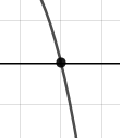
\includegraphics[width = 0.3\textwidth]{../Figures/polyZeroBehaviorAA.png}\item 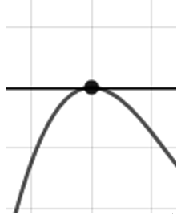
\includegraphics[width = 0.3\textwidth]{../Figures/polyZeroBehaviorBA.png}\item 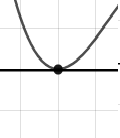
\includegraphics[width = 0.3\textwidth]{../Figures/polyZeroBehaviorCA.png}\item 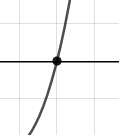
\includegraphics[width = 0.3\textwidth]{../Figures/polyZeroBehaviorDA.png}\end{multicols}\item None of the above.
\end{enumerate} }
\litem{
Construct the lowest-degree polynomial given the zeros below. Then, choose the intervals that contain the coefficients of the polynomial in the form $x^3+bx^2+cx+d$.\[ -2 - 3 i \text{ and } -3 \]\begin{enumerate}[label=\Alph*.]
\item \( b \in [1, 4], c \in [5.44, 8.1], \text{ and } d \in [8.6, 9.7] \)
\item \( b \in [-13, -5], c \in [23.8, 26.58], \text{ and } d \in [-41.4, -37.8] \)
\item \( b \in [1, 4], c \in [3.4, 5.01], \text{ and } d \in [5.2, 6.9] \)
\item \( b \in [2, 15], c \in [23.8, 26.58], \text{ and } d \in [37.2, 41.1] \)
\item \( \text{None of the above.} \)

\end{enumerate} }
\litem{
Construct the lowest-degree polynomial given the zeros below. Then, choose the intervals that contain the coefficients of the polynomial in the form $ax^3+bx^2+cx+d$.\[ -5, -2, \text{ and } 3 \]\begin{enumerate}[label=\Alph*.]
\item \( a \in [-5, 6], b \in [-4.3, -3.7], c \in [-13, -6], \text{ and } d \in [25, 37] \)
\item \( a \in [-5, 6], b \in [1.6, 4.9], c \in [-13, -6], \text{ and } d \in [25, 37] \)
\item \( a \in [-5, 6], b \in [-6.1, -5.4], c \in [-9, 1], \text{ and } d \in [25, 37] \)
\item \( a \in [-5, 6], b \in [-10.9, -9.5], c \in [29, 36], \text{ and } d \in [-30, -23] \)
\item \( a \in [-5, 6], b \in [1.6, 4.9], c \in [-13, -6], \text{ and } d \in [-30, -23] \)

\end{enumerate} }
\litem{
Describe the zero behavior of the zero $x = 4$ of the polynomial below.\[ f(x) = 8(x - 4)^{5}(x + 4)^{8}(x - 8)^{3}(x + 8)^{5} \]\begin{enumerate}[label=\Alph*.]
\begin{multicols}{2}\item 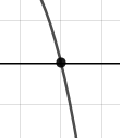
\includegraphics[width = 0.3\textwidth]{../Figures/polyZeroBehaviorCopyAA.png}\item 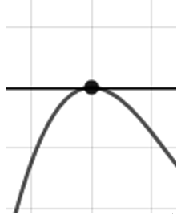
\includegraphics[width = 0.3\textwidth]{../Figures/polyZeroBehaviorCopyBA.png}\item 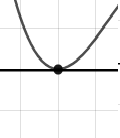
\includegraphics[width = 0.3\textwidth]{../Figures/polyZeroBehaviorCopyCA.png}\item 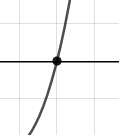
\includegraphics[width = 0.3\textwidth]{../Figures/polyZeroBehaviorCopyDA.png}\end{multicols}\item None of the above.
\end{enumerate} }
\litem{
Describe the end behavior of the polynomial below.\[ f(x) = -7(x + 2)^{3}(x - 2)^{6}(x - 3)^{5}(x + 3)^{7} \]\begin{enumerate}[label=\Alph*.]
\begin{multicols}{2}\item 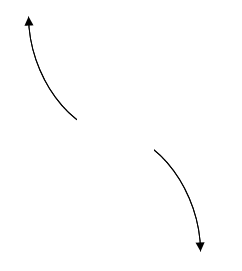
\includegraphics[width = 0.3\textwidth]{../Figures/polyEndBehaviorCopyAA.png}\item 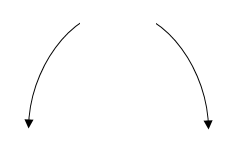
\includegraphics[width = 0.3\textwidth]{../Figures/polyEndBehaviorCopyBA.png}\item 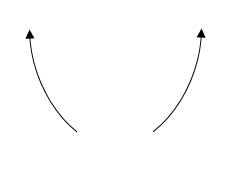
\includegraphics[width = 0.3\textwidth]{../Figures/polyEndBehaviorCopyCA.png}\item 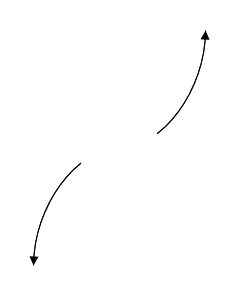
\includegraphics[width = 0.3\textwidth]{../Figures/polyEndBehaviorCopyDA.png}\end{multicols}\item None of the above.
\end{enumerate} }
\litem{
Describe the end behavior of the polynomial below.\[ f(x) = 9(x - 6)^{3}(x + 6)^{8}(x - 7)^{3}(x + 7)^{4} \]\begin{enumerate}[label=\Alph*.]
\begin{multicols}{2}\item 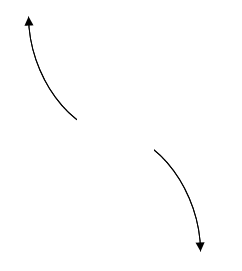
\includegraphics[width = 0.3\textwidth]{../Figures/polyEndBehaviorAA.png}\item 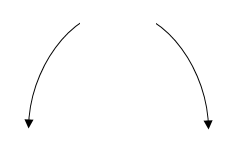
\includegraphics[width = 0.3\textwidth]{../Figures/polyEndBehaviorBA.png}\item 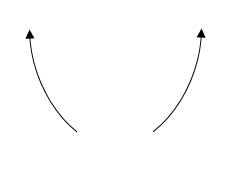
\includegraphics[width = 0.3\textwidth]{../Figures/polyEndBehaviorCA.png}\item 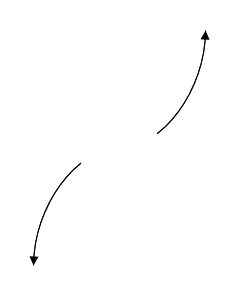
\includegraphics[width = 0.3\textwidth]{../Figures/polyEndBehaviorDA.png}\end{multicols}\item None of the above.
\end{enumerate} }
\litem{
Which of the following equations \textit{could} be of the graph presented below?
\begin{center}
    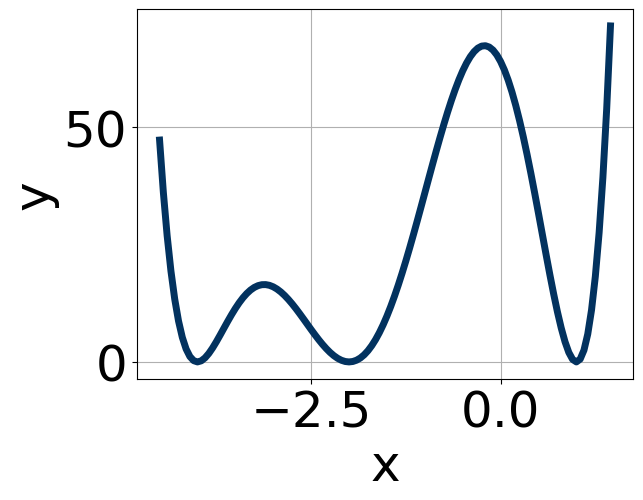
\includegraphics[width=0.5\textwidth]{../Figures/polyGraphToFunctionCopyA.png}
\end{center}
\begin{enumerate}[label=\Alph*.]
\item \( -8(x + 4)^{10} (x + 2)^{10} (x - 1)^{8} \)
\item \( -15(x + 4)^{4} (x + 2)^{10} (x - 1)^{7} \)
\item \( 16(x + 4)^{10} (x + 2)^{8} (x - 1)^{9} \)
\item \( 3(x + 4)^{4} (x + 2)^{5} (x - 1)^{7} \)
\item \( 20(x + 4)^{10} (x + 2)^{8} (x - 1)^{8} \)

\end{enumerate} }
\litem{
Construct the lowest-degree polynomial given the zeros below. Then, choose the intervals that contain the coefficients of the polynomial in the form $x^3+bx^2+cx+d$.\[ 2 - 4 i \text{ and } -3 \]\begin{enumerate}[label=\Alph*.]
\item \( b \in [-0.9, 1.3], c \in [7.04, 8.22], \text{ and } d \in [-63, -58] \)
\item \( b \in [-1.3, 0.3], c \in [7.04, 8.22], \text{ and } d \in [58, 61] \)
\item \( b \in [-0.9, 1.3], c \in [0.36, 1.21], \text{ and } d \in [-9, -1] \)
\item \( b \in [-0.9, 1.3], c \in [6.7, 7.73], \text{ and } d \in [9, 17] \)
\item \( \text{None of the above.} \)

\end{enumerate} }
\end{enumerate}

\end{document}